\subsection{Sewing threads for backpacks} \label{sec:sewing-thread}

When it comes to choosing your thread, there is of course no right or wrong choice. But there are a few things to consider, and then, there is experimentation, trial and error.

For outdoor applications, and more specifically backpacks, you obviously want to consider absolute tensile strength, but it is by far not the only criteria. Resistance to ultraviolet light, exposure to water (fresh water or maybe sea water) and ability to stretch are amongst the important factors. Personally, I also consider how easy to sew a thread is, which is mostly defined by the thread size (together with the choice of needle). In regards to the material, most of the common-man's threads will be either Nylon or Polyester. There are higher quality, higher price threads like PTFE, Dyneema, Kevlar and more but I think this would be beyond the point of building your own packs at home.

\begin{figure}[H]
  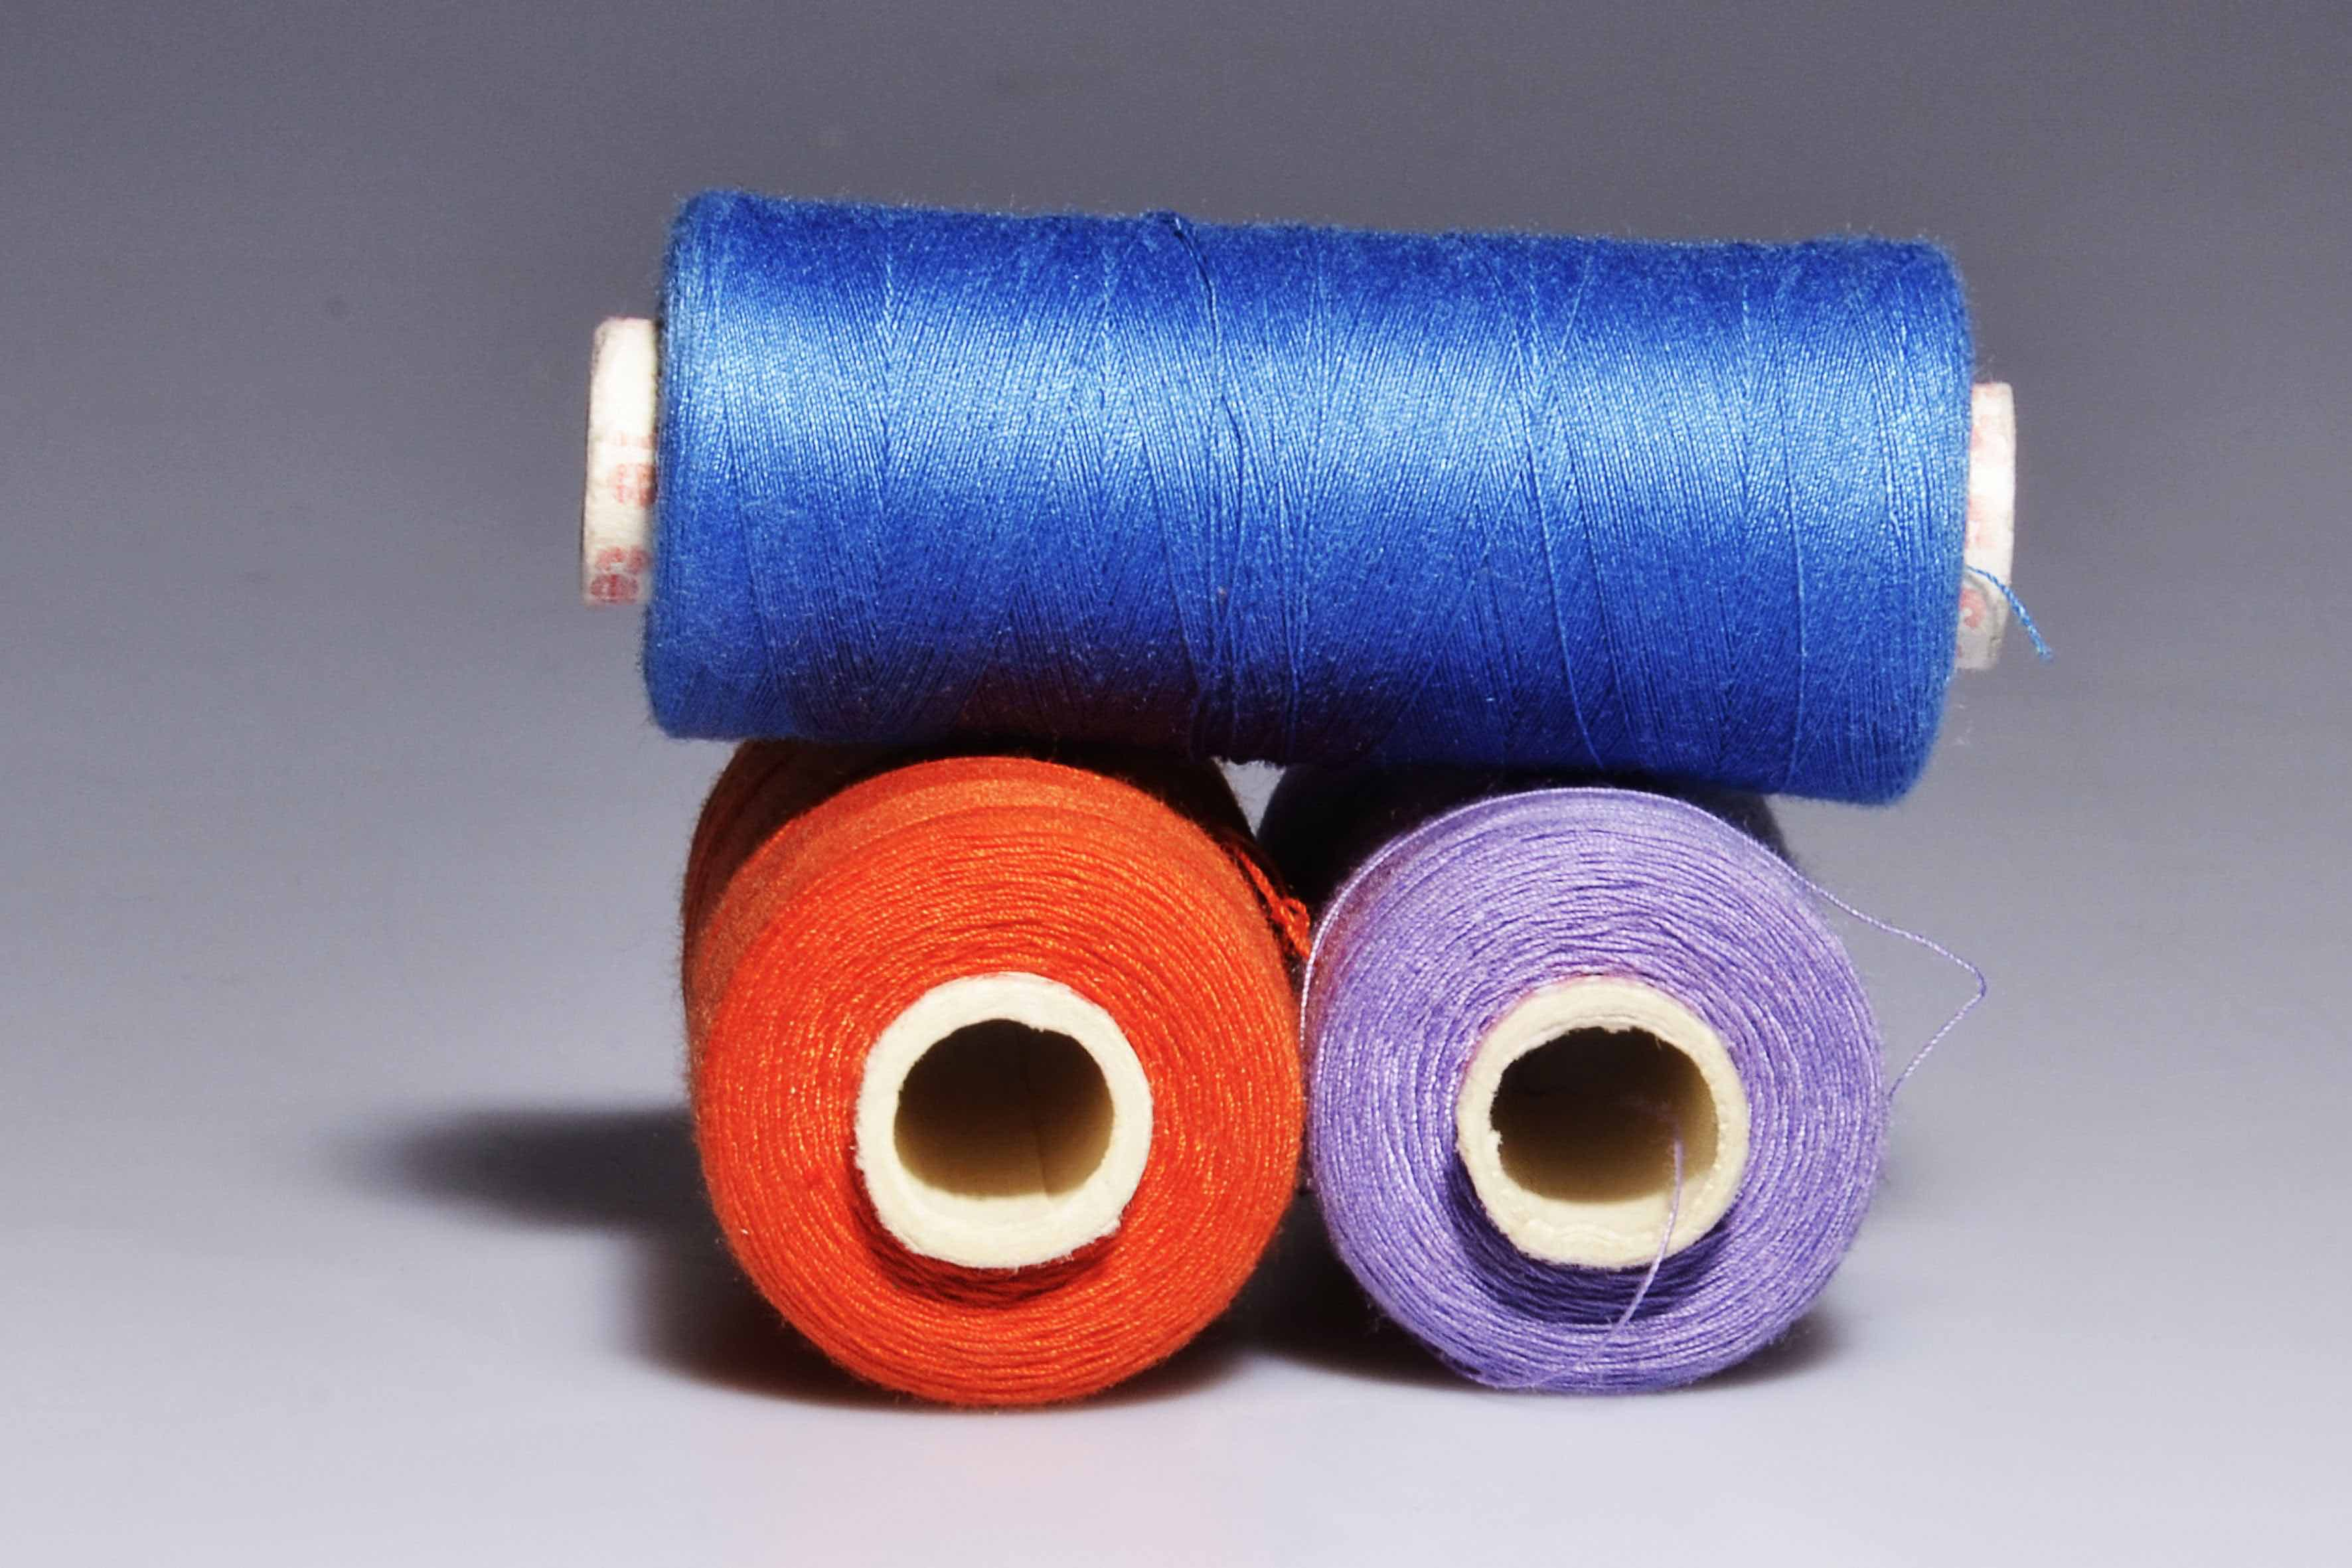
\includegraphics[width=\textwidth]{media/images/place-holder}
  \caption{Illustration of multiple sewing threads}
  \label{img:sewing-threads}
\end{figure}

For its resistance to UV exposure, Polyester is the way to go for durability. As to the thread size, I always prefer triple stitching a thinner thread than having to deal with a cumbersome heavy thread and beefier needles. It allows a higher combined strength than a heavier single stitch, and allows the fabric to stretch under load without snapping. Look at the section \ref{sec:stitching-for-abuse} for more details on how I use such thin threads.

Unfortunately, as there is no universal unit - or any proper conversion system - for thread thickness, I can only give you a tensile strength recommendation and which needle size I use for this particular thread. I use a German-made 100\% polyester thread from Alterfil (the S-100) with a tensile strength of 1570 cN (3.5 pounds of force) with 19\% elongation which is around half the single-stitch tensile strength recommended for a backpack seam ( approx. 3000 cN or 6.7 lbf). The S-100 is working perfectly with a size 90/14 or 100/16 universal needle.

\begin{table}[H]
  \centering
  \begin{tabular}{ | l | l | p{8cm} | }
    \hline
      \textbf{Thread} &
      \textbf{Tensile Strength} &
      \textbf{Recommended use} \\
    \hline
      S-120 &
      1230 cN / 2.76 lbf &
      sports jackets, waistcoats, trousers, coats, jackets, shirts, dresses, sportswear, fabrics of micro-fibre, blouses, underwear/linen, home textiles, curtains, ... \\
    \hline
      S-100 &
      1570 cN / 3.52 lbf &
      outer-wear, sport jackets, waistcoats, trousers, coats, fabrics of micro-fibre, quilting machines \\
    \hline
      S-80 &
      2100 cN / 4.72 lbf &
      jeanswear, sportswear, quilted ornaments, working clothes \\
    \hline
      S-50 &
      3200 cN / 7.19 lbf &
      jeanswear, sportswear, quilted ornaments, working clothes, leather, \textit{rucksacks}, sleeping bags, mattresses, upholstery, hand- and travelling bags \\
    \hline
      S-35 &
      4000 cN / 8.99 lbf &
      jeanswear, quilted ornaments, sportswear, upholstery, \textit{rucksacks} \\
    \hline
  \end{tabular}
  \caption{Alterfil's polyester sewing thread tensile strength recommended use}
\end{table}


\subsection{Stitching for abuse} \label{sec:stitching-for-abuse}

I find it cumbersome to use a heavy-duty thread when sewing together a backpack. Parts of the pack which involve stitching together multiple layers of fabrics can sometime be quite tough on the sewing machine if the needle and thread size are too wide. So I use a thinner thread instead (see \ref{sec:sewing-thread}).

In combination with this, I use a special stitch, often referred to as the triple stretch stitch or backstitch, which is very robust yet flexible but still uses a single thread and a single needle. The result is much stronger than the tensile strength of the thread itself, and its construction has the added benefit of rendering a single point of failure almost impossible. As the triple pass (two time forward, one time backward each step) prevents any snapped thread from getting loose, resulting in a catastrophic failure of your seam.

The backstitch also provides a higher stretching of the seam, resulting in overall less stress on the thread if parts of the pack are under more constraints.
